\section{CNN}



\paragraph{Functionality} The Elsevier article class is based on the standard article class and supports almost all of the functionality of that class. In addition, it features commands and options to format the
\begin{itemize}%\begin{enumerate}[(1)]
\item document style
\item baselineskip
\end{itemize}



\begin{figure}
    \centering
    \begin{minipage}[b]{.5\textwidth}
        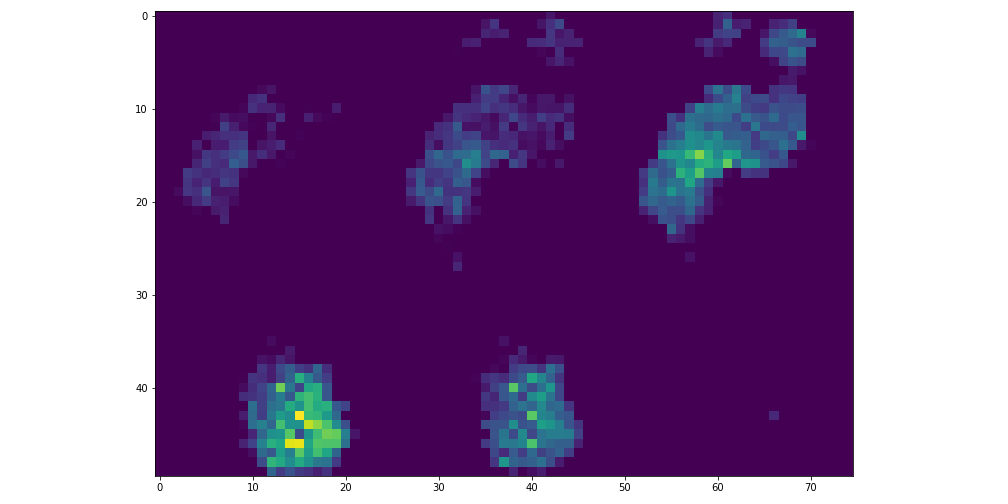
\includegraphics[width=\textwidth]{figures/project/frame1.png}
    \end{minipage}
    \caption{sample image.}
    \label{fig:Stepscan_dataset}
\end{figure}


Here are two sample references: \cite{SKazemii/EE6563}.